% Chapter 1
% 
\chapter{Introdução} % Main chapter title
\label{chap:Introdução} % For referencing the chapter elsewhere, use Chapter~\ref{Introdução}

Neste capítulo inicial, é fornecido ao leitor um contexto amplo, facilitando a interpretação dos assuntos descritos ao longo deste relatório.

A introdução organiza-se em torno do enquadramento e do contexto do projeto. Nele apresentam-se os aspetos iniciais essenciais: o problema em estudo, os objetivos e a abordagem adotada. Por fim, o capítulo explicita os contributos do projeto, o planeamento e a estrutura geral do relatório.




%-------------------------------------------------------------------------------
%---------
%
\section{Enquadramento/Contexto} 
\label{sec:chap1_introduction} %For referencing this section elsewhere, use Section~\ref{sec:chap1_introduction}
O presente projeto surge no âmbito da \gls{UC} \gls{PESTI}
da Licenciatura em Engenharia Informática do Instituto Superior de Engenharia do Porto e
foi desenvolvido no escritório da \textit{OnlyHighIQ}.

Este projeto parte de uma interpretação rigorosa do problema e aplica os conhecimentos adquiridos e as boas práticas de engenharia informática. Sintetiza o estado da arte e compara abordagens alternativas. Após esta avaliação, desenha-se e implementa-se a solução, sustentada por testes e documentação. Por fim, registam-se e apresentam-se com rigor os processos, decisões e resultados.

A \textit{OnlyHighIQ} é uma empresa fundada recentemente, encontra-se no coração da cidade do Porto, a sua localização oferece um enquadramento dinâmico e inspirador à inovação e à colaboração. Inserida numa zona vibrante, reconhecida pela sua rica história e relevância cultural, a área garante acesso facilitado a comodidades essenciais e às principais ligações de transporte, constituindo um polo conveniente para clientes e parceiros. \cite{OYI}

A missão, a visão e os valores são os pilares fundamentais para definir a identidade e o propósito de uma organização.


\begin{table}[H]  % «H» = exatamente aqui
\caption{Missão, Visão e Valores da OnlyHighIQ}
\label{tab:missao_visao_valores}
\begin{center}
\begin{tabular}{|l|p{10cm}|}
\hline
\textbf{Missão} & "...\textit{to create a dynamic community where brilliant minds collaborate to develop cutting-edge solutions and innovative platforms that transform visionary ideas into reality.}" \cite{OYI} \\ \hline
\textbf{Visão} & "\textit{To create a limitless innovation landscape where the most brilliant minds, have the tools to build the future—ensuring that progress and opportunity are distributed to everyone, everywhere.}" \cite{OYI} \\ \hline
\textbf{Valores} & "\textit{Innovation Without Borders, Collaborative Excellence, Impact with Purpose, Courage to Disrupt, Principle-Led Integrity}" \cite{OYI} \\ \hline
\end{tabular}
\end{center}
\end{table}

A \textbf{OnlyYes} é o seu primeiro projeto que surge como ecossistema principal da empresa mãe, o seu foco é principalmente na criação de conteúdo pago. 

Neste relatório vão ser focados aspetos da propagação de conteúdo de baixa latência, mas é importante realçar que a solução implementada passa por toda a infraestrutura. A solução apresentada neste relatório, foi apenas uma etapa entre vários processos e componentes, e decisões que levarão a \textbf{OnlyYes} ao lançamento.

O meu percurso na \textbf{OnlyHighIQ} decorreu durante cerca de quatro meses, período em que fui instruído de planear, conceber e discutir a arquitetura global da aplicação, de acordo com as boas práticas transmitidas na formação \textbf{\textit{AWS Cloud Architect}} ministrada pela empresa, bem como com os padrões e conhecimentos que fui adquirindo ao longo do meu percurso.


\section{Descrição do Problema} \label{Problema}

Atualmente, no mercado de criação de conteúdo encontram-se diversas barreiras técnicas para pessoas com dificuldades tecnológicas. Muitos dos criadores de conteúdo, dependem de ferramentas externas para realizar uma transmissão ao vivo, então a \textbf{OnlyYes} quer implementar uma rede social, onde seja possível realizar uma \textit{livestream} com poucos cliques e pré-requisitos.

Apontou-se, também, a necessidade dos criadores de conteúdo conseguirem comunicar com os utilizadores da plataforma, pelo que foi necessário realizar um \textit{low latency chat}.

O problema resume-se à criação de uma experiência unificada de \textit{livestream} e comunicação em tempo real, acessível em poucos cliques, sem depender de ferramentas externas.
 

\subsection{Objetivos} 

Para a solução a desenvolver, definiu-se os seguintes objetivos:
\begin{itemize}
    \item \textbf{Modelação e criação de escalões de acesso para controlar o acesso à transmissão}: após a criação do perfil privado, são criados escalões com diferentes preços e benefícios.
    \item \textbf{Criação de canal único por criador}: provisionar um canal exclusivo a cada criador.
    \item \textbf{Desenvolvimento da interface do criador}: \textit{dashboard} para iniciar e terminar a transmissão, escolher câmara e microfone, pré-visualizar o vídeo, definir título e descrição, editar um menu de doações, e visualizar métricas.
    \item \textbf{Desenvolvimento da interface do utilizador}: página de visualização com \textit{player} (\textit{play}/pausa, \textit{mute}, volume, ecrã inteiro, seleção de qualidade), com um menu de doações definido pelo criador.
    \item \textbf{Garantia a privacidade do Criador}: capacidade de controlar o acesso à câmara e ao microfone.
    \item \textbf{Implementação do \textit{chat} em direto}, permite enviar mensagens para cada utilizador durante a transmissão, incluindo o criador.
\end{itemize}

Estes foram os objetivos traçados para este projeto, que serviu para integrar o \gls{MVP}

\subsection{Abordagem} 

Para realizar os objetivos deste projeto a empresa incutiu uma metodologia ágil, que facilita a comunicação e a resolução de problemas em equipa. A metodologia \textbf{SCRUM} é considerado uma \textit{framework} de desenvolvimento de \textit{software}.

\begin{figure}[H]
\centering
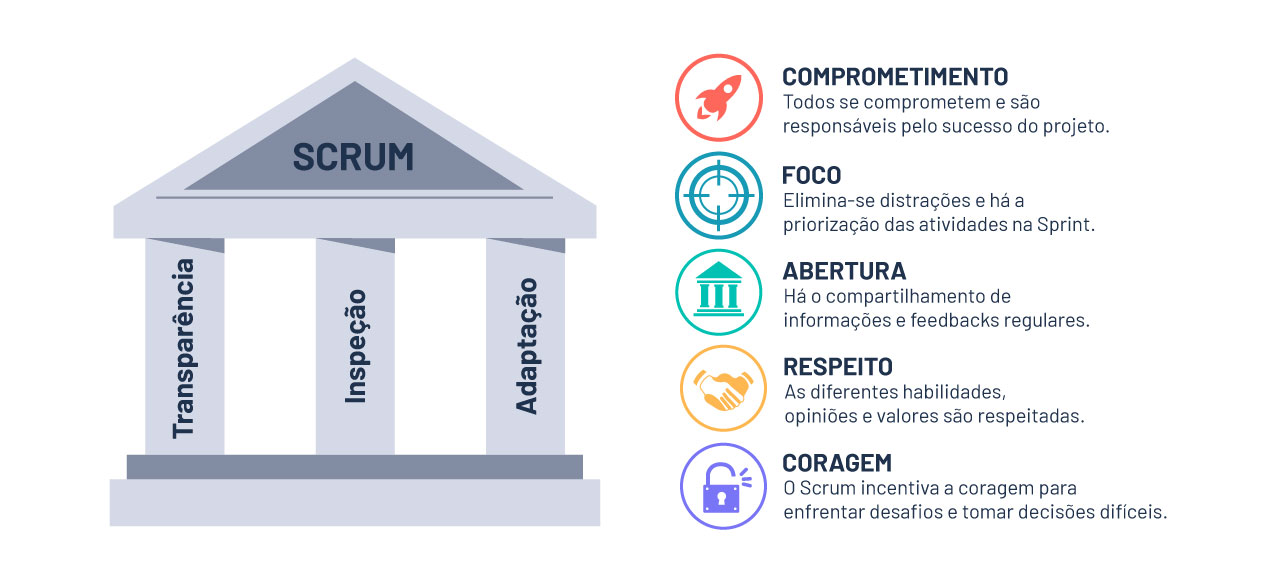
\includegraphics[width=0.8\textwidth]{frontmatter/assets/scrumMethodology.jpg}
\caption{Pilares e Valores Da Metodologia SCRUM \cite{Espinha2024ScrumArtia}}
\label{fig}
\end{figure}

Para o projeto foi essencial seguir os pilares da metodologia: \textbf{Transparecia}, \textbf{Reflexão} (Inspeção), e \textbf{Adaptação}. A metodologia não serve apenas e só para a coordenação do projeto, mas os seus valores devem ser seguidos, independentemente do local de trabalho.


"Scrum is an incremental and iterative agile software development framework for managing product development (...) This strategy challenges assumptions of the "traditional, sequential approach" to product
development, and encourages teams to self-organize by encouraging close online collaboration of all team
members, as well as face-to-face communication among all team members and disciplines in the project.(...)"\cite{Sachdeva2016Scrum}

A implementação do \textbf{SCRUM} no projeto para além do descrito, foi feita através de \textit{Sprints}. Os sprints são espaços de tempo definidos para mostrar as evoluções ao cliente do projeto a desenvolver. Para além disso foram realizadas \textit{daily meetings} que permitiram verificar o processo de cada membro da equipa e avaliar o progresso do projeto como um todo.


\subsection{Contributos} 

\textbf{Tecnológicos}: Entrega de uma solução de \textit{streaming} ligado a um controlo de acesso por \textit{tiers}, um \textit{player} simples e responsivo, com \textit{chat} de baixa latência. Adoção de práticas \gls{CI/CD} e controlo de versões.

\textbf{Organizacionais}. Redução da dependência de ferramentas externas e consolidação da experiência de \textit{streaming} na própria plataforma, aumentando a capacidade de controlo e a qualidade da interação do criador com a sua comunidade.

\textbf{Pedagógicos}. Consolidação de competências em desenho arquitetural, integração de componentes em tempo real e entrega orientada a \gls{MVP}, com documentação e avaliação objetiva do resultado.     

\paragraph{Síntese dos contributos}
\begin{itemize}
    \item Criação de uma plataforma de \textit{streaming} com canais exclusivos por criador.
    \item Controlo a canais exclusivos por \textit{tiers} e integração com subscrições e pagamentos.
    \item Disponibilização de um \textit{player} responsivo e simples (play/pausa, volume, ecrã inteiro, seleção de qualidade).
    \item \textit{Chat} de baixa latência, com texto e emojis, suportado por \textit{API WebSocket}.
    \item Mecanismos de privacidade e segurança
    \item Adoção de boas práticas de engenharia (\gls{CI/CD}, controlo de versões com uso de \textit{branching}, testes automáticos...).
    \item Crescimento técnico e profissional da individual e da equipa, com aplicação prática de tecnologias não abordadas em contexto académico.
\end{itemize}


\subsection{Planeamento do trabalho}  

Durante o estágio, o desenvolvimento da solução decorreu em etapas bem definidas. Numa fase inicial, realizou-se uma pesquisa com duração aproximada de duas semanas. Concluída essa etapa, a equipa avançou para o planeamento de \gls{UC's} e \gls{US}, formalizando critérios e dependências. Seguiu-se a fase de arquitetura, durante a qual foram elaboradas as vistas lógicas, de implementação e físicas, os diagramas de sequência, o modelo de domínio e de dados, bem como a seleção das tecnologias e dos sistemas de gestão de bases de dados. Esta fase inicial estendeu-se por cerca de quatro semanas. Por fim, o supervisor organizou o trabalho em \textit{sprints} de duas semanas no Jira, distribuindo as tarefas até à entrega da solução.

Durante os \textit{sprints}, a equipa seguiu o formato \textit{SCRUM} com \textit{daily meetings}. A implementação foi organizada em fases sequenciais, a partir do desenho produzido na fase de arquitetura, criou-se a camada de domínio e a base de dados. Em seguida, desenvolveram-se as operações \gls{CRUD} e os serviços nucleares de \textit{back-end}, prosseguiu-se com a interface de utilizador e de criador, bem como as integrações, por fim, construíram-se as funções \textit{AWS Lambda} e efetuou-se a ligação \textit{front-end}/\textit{back-end}, finalizado em afinações e testes do \gls{MVP}. A Tabela~\ref{tab:tempo_projeto} sintetiza esta distribuição temporal.


\begin{table}[H]  % «H» = exatamente aqui
\caption{Divisão de tempo no projeto}
\label{tab:tempo_projeto}
\begin{center}
\begin{tabular}{|l|p{10cm}|}
\hline
\textbf{Período de Tempo} & \textbf{Tarefa} \\ \hline
24/02 a 07/03 & Período de pesquisa \\ \hline
10/03 a 21/03 & Fase de arquitetura \\ \hline
24/03 a 04/04 & \textbf{Sprint 1} - Criação das classes de domínio, bases de dados, e preparar o ambiente local \& Inicio da pesquisa para o relatório \\ \hline
07/04 a 18/04 & \textbf{Sprint 2} - Desenvolvimento do \gls{CRUD} \\ \hline
05/05 a 16/05 & \textbf{Sprint 3} - Desenvolvimento dos serviços principais de \textit{Back-End} \& Realização dos estado da arte \\ \hline
19/05 a 30/05 & \textbf{Sprint 5} - Desenvolvimento da interface de utilizador e criador \\ \hline
02/06 a 13/06 & \textbf{Sprint 6} - Criação das lambdas e ligação entre o Front-End e Back-End \\ \hline
16/06 a 22/06 & \textbf{Sprint 7} - Afinações e testes para o \gls{MVP} \\ \hline
23/06 a 10/09 & Continuação da realização do relatório. \\ \hline
\end{tabular}
\end{center}
\end{table}




\section{Estrutura do relatório}


Para além da introdução, este documento contém mais 4 capítulos, que apresentam as várias etapas do desenvolvimento da solução. 

No capítulo \ref{chap:EA}, é descrito o estado da arte e são apresentados trabalhos relacionados. No capítulo \ref{chap:ADS}, o planeamento e o desenho, que foram previamente concebidos com a equipa para um melhor enquadramento no projeto como um todo. É realçado o domínio bem como os requesitos funcionais e não funcionais No capítulo \ref{chap:Impl}, são detalhados os vários processos de implementação da solução, onde constam exemplos de funcionalidades, testes para a validação do projeto e imagens com a interface de utilizador. Por fim, o capítulo \ref{chap:Conc}, concentra-se nos resultados obtidos, e numa introspeção final da solução e do relatório.

\vspace{20mm} 
